\documentclass{article}

\usepackage{graphicx}
\usepackage{caption}
\usepackage{multicol}
\usepackage{amssymb}
\usepackage[margin=0.5in]{geometry}
\usepackage{ragged2e}
\usepackage{boondox-cal}
\renewcommand{\vec}[1]{\mathbf{#1}}

\begin{document}

\title{Dependencies of Ferromagnetism and Paramagnetism based on the Ising Model}
\author{Joseph Spear}

\maketitle


\begin{abstract}
\justify
The study of statistical mechanics in thermodynamics allows for the calculation of various thermodynamic properties. Some materialistic properties such as Heat Capacity and Magnetic Susceptibility can be found, as well as the dependencies of the system's Energy and Magnetization as functions of the temperature or external magnetic field. The system of atoms are modeled using the Ising Model, and the various quantities are approximated using the Monte-Carlo method. These approximations yield results based on the Curie Temperature, and allow for the quantities to be found graphically.
\end{abstract}

\begin{multicols}{2}
\section{Introduction}
The introduction of a statistical view of thermodynamics begins with the Kinetic Theory of Gases, developed by Daniel Bernoulli in 1738. (Uffink, 6-8) This was refined by James Clerk Maxwell, developing the Maxwell Distribution, which was the first statistical law in physics. Maxwell's work was developed further by Boltzmann in his \textit{Lectures on Gas Theory} (Ebeling, Werner; Sokolov, Igor M.) in 1896, and Gibbs in 1902 with the publication of \textit{Elementary Principles in Statistical Mechanics}. 

\subsection{Ising Model}
Eventually, the ferromagnetic properties in various materials were explored and this gave rise to what is now known as the "Ising Model". Originally created by  Wilhelm Lenz, he gave topic to his student Ernst Ising who would develop it in one dimension and two dimensions. The two-dimensional Ising Model is set of lattice points representing atoms in a material. Each lattice point has adjacent neighbors which interact with the atom in question. The energy and magnetization of this system can be calculated using statistical methods, but it may also be approximated using what is known as the Monte-Carlo Method.

\subsection{Monte-Carlo Method}
There are multiple different algorithms to use the Monte-Carlo method, however, the most common is the Metropolis algorithm. The Metropolis algorithm is implemented by first generating a random spin configuration of the lattice (defining the spin for every lattice point in the lattice) and then randomly flipping the spin of one of the atoms in the lattice from a positive to negative or vice versa. This perturbation is then checked, keeping the new spin configuration if a certain desired criteria is met, and undoing the perturbation if it is not. 

The process is then repeated a large number of times until successive iterations yield very small changes in the quantity in question. This step is known as the "Burn In" step, and is used to get rid of any data that is initially largely inaccurate. At this point, the process continues recording the desired data with much greater accuracy than the data generated in the burn in. Figure 1 shows an example of this process using the Energy of a 25 by 25 lattice which is perturbed until reaching a stable value. 

\begin{center}
\includegraphics[width=3.58in]{EvsIterations_100000_Steps.eps}
\scriptsize{
Figure 1: Change in Energy after 100000 Steps
}
\end{center}

Here it is clear that the Energy values stabilize around 25,000 iterations. To be ensure accuracy, recording begins around 50,000 iterations and the "Burn In" step ends.

\section{Implementation}
In order to implement the Metropolis Monte-Carlo Method, it is necessary to generate a completely random spin configuration to begin with, as well as randomly picking a lattice point to perturb. This may be done with the built in GFORTRAN calls of \verb!random_seed! and \verb!random_number! which will provide a random initial configuration and perturbation as needed. 

To simplify the implementation, the Ising Model will assume the shape of a square. To represent the Ising Model, a two dimensional array is used with size \verb!size = 25! will be allocated. To set up the initial conditions, a random number ($0 < randNum < 1$) is generated. If the number is less than or equal to $0.5$ then it will assign a $-1$ to that lattice point, otherwise it will assign a $1$ to the lattice point. Once this random configuration is produced, then a random lattice point will be chosen and have it's spin flipped, perturbing the configuration. The change in Energy is calculated then the process is done repeatedly until the energies stabilize as in Figure 1. Once the values stabilize, they are recorded and the average is found by using the algorithm below. 

\begin{verbatim}

do n = 1, bigNum2
  call random_number(tmp)
  ri = floor(tmp*size) + 1
  call random_number(tmp)
  rj = floor(tmp*size) + 1
        
  spin(ri, rj) = -spin(ri, rj)
  DE = -2.0 * J * (spin(mod(ri, size)+1, rj) &
  + spin(ri, (mod(rj, size)+1)) + spin(mod &
  (ri+size-2, size)+1,rj) + spin(ri, &
  (mod(rj+size-2, size)+1))) * &
  spin(ri, rj) - Mu * B * spin(ri, rj)
  if (DE < 0) then
  E = E + DE
  M = M + 2* spin(ri, rj)
  else 
    call random_number(tmp)
    if(tmp < exp(-DE/(k*T))) then
      E = E + DE
      M = M + 2*spin(ri, rj)
    else
      spin(ri, rj) = -spin(ri,rj)
      SumE = SumE + E
      SumE2 = SumE2 + E*E
      SumM = SumM + abs(M)
      SumM2 = SumM2 + M*M
    end if
  end if

end do

AvgE = SumE/bigNum2
AvgE2 = SumE2/bigNum2
AvgM = SumM/bigNum2
AvgM2 = SumM2/bigNum2

heatCap = (1.0/(k*T*T)) * (AvgE2-AvgE*AvgE)
susceptibility = (AvgM2 - AvgM*AvgM)/(k*T)

\end{verbatim}

In the above code, \verb!spin! is the two dimensional spin configuration, \verb!E! is the Energy of the state for each iteration, \verb!M! is the Magnetization of the state for each iteration, \verb!B! and \verb!T! are the variable external magnetic field and temperature respectively. \verb!J! is the interaction energy and can be found using the equation:

\begin{equation}
    \label{equation1}
    		J = \frac{1}{2} T_c k \hspace{0.02in} ln\left(1 + \sqrt{2}\right)
\end{equation}

\vspace{0.1in}

The \verb!AvgE! can be calculated using the Conatical Distribution as follows:

\begin{equation}
    \label{equation2}
    \bar{E} = \sum \frac{E_r \cdot e^{-\frac{E}{k_BT}}}{e^{-\frac{E}{k_BT}}}
\end{equation}

\vspace{0.1in}

however, with the use of the Monte-Carlo method, it is approximated. 

\section{Results}
\subsection{Ferromagnetism}
When computing the Energies and Magnetization of a ferromagnetic material, it is important to vary the values across temperature and an external magnetic field. By doing this, various quantities, such as the Curie temperature, the heat capacity, and the magnetic susceptibility may be found. Figure 2 shows the Energy as a function of temperature using 500,000 iterations and a constant magnetic field of $B=10$.

\begin{center}
\includegraphics[width=3.58in]{2EvsT_B_Equal_10.eps}
\scriptsize{
Figure 2: Energy as a function of the Temperature.
}
\end{center}

The Magnetization as a function of temperature is shown in Figure 3 with the same parameters as that of Figure 2:

\begin{center}
\includegraphics[width=3.58in]{MvsT_B_Equal_10.eps}
\scriptsize{
Figure 3: Magnetization as a function of the Temperature.
}
\end{center}

From observing Figures 2 and 3, many characteristics of ferromagnetic materials can be determined. While the \verb!J! was determined in this program from the Curie temperature of Iron ($T_c = 1043.2$), if it had been determined a different way, then the inflection point on Figure 2 and 3 would provide the $T_c$ since it is defined as the point at which the ferromagnetic properties break down. The loss of Magnetism with high temperatures is observed in Figure 3, explaining the phenomenon that is observed in the natural world. 

Other quantities such as the Heat Capacity and the Magnetic Susceptibility are also able to be found computationally. To approximate the Average Heat Capacity, equation 3 is used:

\begin{equation}
    \label{equation3}
    C_v = \frac{1}{kT^2} \left(<\bar{E}^2> - <\bar{E}>^2\right)
\end{equation}

\vspace{0.1in}

When the average Heat Capacity is graphed over various temperatures, the actual Heat Capacity of the material is found at the peak of Figure 4:

\begin{center}
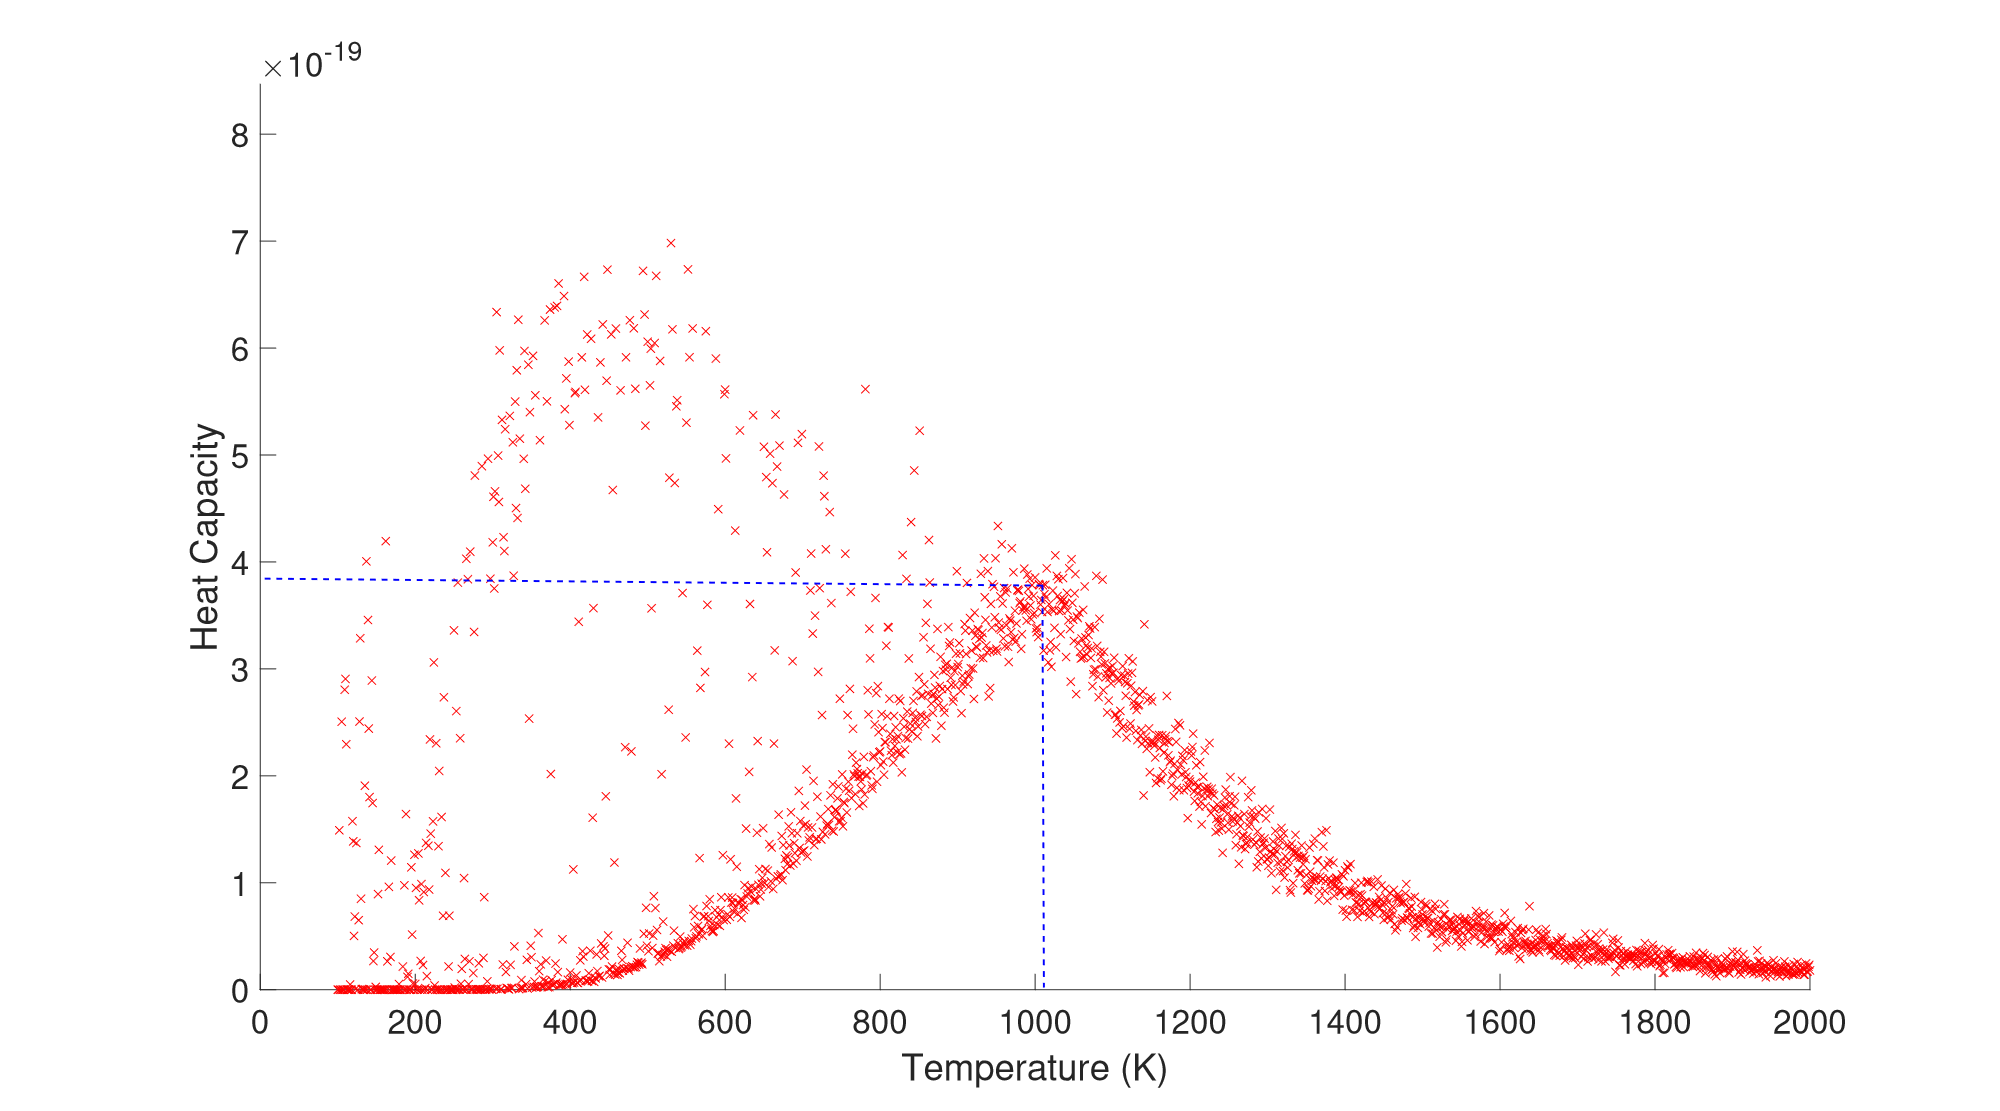
\includegraphics[width=3.58in]{HC.eps}
\scriptsize{
Figure 4: Heat Capacities with different Temperatures.
}
\end{center}

located at the Curie temperature, the Heat Capacity is roughly $3.85\times 10^{-19} \frac{J}{Atom \cdot K}$ based on the results of the Monte-Carlo method. To approximate the Magnetic Susceptibility of a material, equation 4 is used:

\begin{equation}
    \label{equation4}
    \chi = \frac{1}{kT}\left(<\bar{M}^2> - <\bar{M}>^2\right) 
\end{equation}

\vspace{0.1in}

When the average Magnetic Susceptibility is graphed over various temperatures, the actual Magnetic Susceptibility of the material is found at the peak of Figure 5:

\begin{center}
\includegraphics[width=3.58in]{MS.eps}
\scriptsize{
Figure 5: Magnetic Susceptibilities with different Temperatures.
}
\end{center}

The Magnetic Susceptibility is found at the peak at the Curie Temperature yet again, and it is found that the Magnetic Susceptibility is roughly $3.05 \times 10^{24}$.

Holding the Temperature at the Curie Temperature and varying the External Magneic Field yields Energies and Magnetization found in Figures 6 and 7:

\begin{center}
\includegraphics[width=3.58in]{EvsB_T_Equal_1200.eps}
\scriptsize{
Figure 6: Energies with varying Magnetic Fields.
}
\end{center}

\begin{center}
\includegraphics[width=3.58in]{MvsB_T_Equal_1200.eps}
\scriptsize{
Figure 7: Energies with varying Magnetic Fields.
}
\end{center}

This shows that on small scales, the Energy and Magnetization is roughly constant with changing external magnetic fields.

\subsection{Paramagnetism}
Para-magnetic materials are those in which they do not retain a net Magnetization. While they do exhibit magnetic properties when an external magnetic field is applied, these properties dissipate very rapidly once the external magnetic field is removed, unlike Ferro-magnets which retain their Magnetization long after the external magnetic field has been removed.

For using the Monte-Carlo method, this is done by setting the interaction equal to 0 ($J = 0$), and the rest remains the same. The difference between Para-magnets and Ferro-magnets when observing Figures 8 through 11.

\begin{center}
\includegraphics[width=3.58in]{EvsT_B_Equal_10_PARA.eps}
\scriptsize{
Figure 8: Energies with varying Temperatures for a Para-magnet.
}
\end{center}

\begin{center}
\includegraphics[width=3.58in]{MvsT_B_Equal_10_PARA.eps}
\scriptsize{
Figure 9: Magnetization with varying Temperatures for a Para-magnet.
}
\end{center}

Figure 8 and 9 show that the Energy and Magnetization associated with the Para-magnetic material decays greatly with temperature. The external magnetic field is held constant at $B = 10H$.

\vspace{1.1in}

\begin{center}
\includegraphics[width=3.58in]{EvsB_T_Equal_1043_PARA.eps}
\scriptsize{
Figure 10: Energies with varying External Magnetic Fields for a Para-magnet.
}
\end{center}


\begin{center}
\includegraphics[width=3.58in]{MvsB_T_Equal_1043_PARA.eps}
\scriptsize{
Figure 11: Magnetization with varying External Magnetic Fields for a Para-magnet.
}
\end{center}

Figure 10 and 11 shows the properties being affected drastically by the changing external magnetic field. The Temperature is held constant at $T = T_c = 1043.2 K$ and shows how both the Energy and Magnetization approach zero as the external magnetic field approaches zero. This is what would be expected, as the magnetic properties disappear with the external magnetic field, taking with it the associated energies.

\section{Conclusion}
While the Metropolis Monte-Carlo method is centered around the use of pseudo-random numbers, the method is fairly consistent with approximating the solution to  the Ising Model. By allowing for a fair amount of iterations to proceed before recording data, the inaccurate approximations can be eliminated, and by letting enough iterations proceed, this may be done consistently. 

Once the Monte-Carlo method is performed, various different properties of any material may be found, such as the Heat Capacity, Magnetic Susceptibility, and Curie Temperatures along with a graphical representation of the Energy and Magnetization's dependencies on Temperature and External Magnetic Field. 

\end{multicols}

\section{References}

\begin{enumerate}

\item Uffink, Jos (2006). Compendium of the foundations of classical statistical physics (Doctoral dissertation).

\item Torquato, Salvatore IOPScience, 2011, https://iopscience.iop.org/article/10.1088/1478-3975/8/1/015017. Accessed 6 Nov. 2019.

\item Ebeling, Werner; Sokolov, Igor M. (2005). Statistical Thermodynamics and Stochastic Theory of Nonequilibrium Systems. Statistical Thermodynamics and Stochastic Theory of Nonequilibrium Systems. Edited by Ebeling Werner \& Sokolov Igor M. Published by World Scientific Press. Series on Advances in Statistical Mechanics. 8. pp. 3–12. Bibcode:2005stst.book.....E. doi:10.1142/2012. ISBN 978-90-277-1674-3. (section 1.2)

\item Griffiths, David J.\textit{Introduction to Electrodynamics: Fourth Edition} United States, Pearson Education, Inc., 2013 

\item Fitzpatrick, Richard \textit{The Ising Model}, 2006, http://farside.ph.utexas.edu/teaching/329/lectures/node110.html. Accessed 7 Nov. 2019.

\end{enumerate}


\end{document}
